\documentclass[12pt]{exam}
\usepackage{amsthm}
\usepackage{libertine}
\usepackage[utf8]{inputenc}
\usepackage[margin=1in]{geometry}
\usepackage{amsmath,amssymb}
\usepackage{multicol}
\usepackage[shortlabels]{enumitem}
\usepackage{siunitx}
\usepackage{cancel}
\usepackage{caption}
\usepackage{graphicx}
\usepackage{pgfplots}
\usepackage{listings}
\usepackage{tikz}


\pgfplotsset{width=10cm,compat=1.9}
\usepgfplotslibrary{external}
\tikzexternalize

\newcommand{\class}{Laboratorio Física II} % This is the name of the course 
\newcommand{\examnum}{Laboratorio 12} % This is the name of the assignment
\newcommand{\examdate}{22/11/2022} % This is the due date
\newcommand{\timelimit}{}
\newenvironment{Figura}
  {\par\medskip\noindent\minipage{\linewidth}}
  {\endminipage\par\medskip}




\begin{document}
\pagestyle{plain}
\thispagestyle{empty}

\noindent
\begin{tabular*}{\textwidth}{l @{\extracolsep{\fill}} r @{\extracolsep{6pt}} l}
\textbf{\class} & \textbf{Name:} & \textit{David Pachon Ballen}\\ %Your name here instead, obviously 
\textbf{\examnum} &&\textit{Sergio Montoya Ramírez}\\
\textbf{\examdate} &&\\
\end{tabular*}\\
\rule[2ex]{\textwidth}{2pt}
% ---


\begin{multicols}{2}
\section{Objetivos}
\begin{itemize}
\item Estudiar el efecto de un campo magnético sobre un
  conductor por el cual circula una corriente eléctrica.
\item Determinar la relación entre la fuerza que experimenta un conductor debido a un campo magnético en
    función de la corriente que circula por él.
\item Medir el campo magnético promedio generado por un
  conjunto de imanes.
\end{itemize}
\section{Introducción}
En este experimento se estudia el efecto de un campo
magnético sobre un conductor por el que pasa una corriente eléctrica. Dicho estudio se hace midiendo los cambios de
fuerza ejercida sobre un soporte plástico por medio de una
balanza. El campo magnético constante es generado por
un conjunto de imanes de neodimio ubicados estratégicamente dentro del soporte de plástico.

  En la primera parte de la práctica se estudiará cualitativamente el campo magnético y sus características. Posteriormente, se estudiará cómo este campo genera una fuerza
sobre el conductor. Se desea que el estudiante comprenda
cómo se usa la regla de la mano derecha para determinar
la dirección de la fuerza ejercida a partir de las direcciones del campo magnético y de la corriente que circula
  por el conductor. Después, se analiza la dependencia de
la magnitud de la fuerza en función de las intensidades
del campo magnético y de la corriente, la cual será una
estimación debida a los caminos irregulares que sigue la
corriente.
\section{Analisis Cualitativo}
\begin{enumerate}
\item Explique, bajo premisas razonables sobre cómo se distribuyen las líneas de campo magnético generadas por
    los imanes y del porqué no se tiene en cuenta los caminos conductores verticales para el cálculo de la fuerza
    que ejerce el campo sobre una baquela.

    Sean A y B los dos lados verticales de la baquela, entonces, por la caracteriztica de las mismas generan un campo magnetico que obedece a \textit{La ley de la mano derecha}. Ahora bien, consideremos la ecuación (12.1) en donde se muestra que la fuerza del campo depende de los vectores $\vec{L}$ y $\vec{B}$ y dado que el campo $\vec{B}$ es el mismo en ambos casos pero los vectores $\vec{L_1},\vec{L_2}$ son paralelos entonces nos queda que sus fuerzas son opuestas y en magnitud iguales por tanto se cancelan mutuamente.

\item Indique en dónde la suposición de campo magnético
  homogéneo inducido por los imanes falla.
    
Como se sabe, la densidad del campo magnetico varia con respecto a la distancia. Por tanto, si nos alejamos o acercamos lo suficiente a alguno de sus polos sus efectos variaran y por tanto no sera homogeneo. Ademas, este no toma en consideración los efectos que otros imanes puedan llegar a tener dado que el campo magnetico es infinito y por tanto si otro iman se acerca lo afectaria.
\item Si la masa del sistema no cambia en todo el procedimiento, ¿qué mide realmente la balanza electrónica?Use la tercera ley de Newton para justificar

  La balanza en general esta midiendo la normal. Esto funciona muy bien cuando hay solo una fuerza (Ya que esta es la reacción) pero como en este caso la fuerza tambien interactua con el campo magnetico podria darse el caso de que estas se restren y destruyan.

\item ¿Es posible que el campo magnético generado por la
  corriente que pasa por los caminos conductores altere el campo magnético de los imanes? Si es así, ¿cómo sería?
    
    Si lo afecta pues al final son cargas moviendose lo cual genera un campo magnetico. Sin embargo, esto el unico efecto real que tiene es aumentar el campo total.

\item Usando la ley de la mano derecha, determine la dirección de la corriente en el camino conductor.

Como suponemos la corriente sale del positivo entonces ese es nuestro a y como en nuestro caso la dirección que funcionó es con la positiva mas a la izquierda entonces el valor de su campo magnetico tenia sentido positivo en y o lo que es lo mismo se dirigia hacia nosotros.
\end{enumerate}
\section{Analisis Cuantitativo}
\begin{Figura}
    \centering
    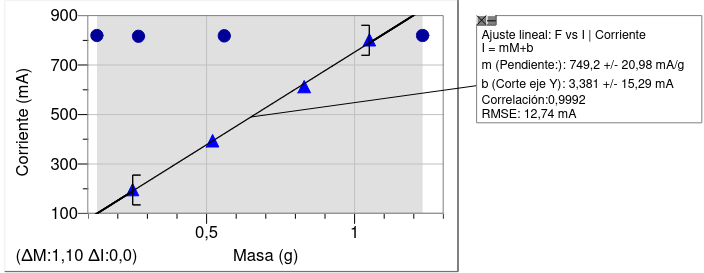
\includegraphics[width=0.9\textwidth]{Img/Figura1_Lab12.png}
    \captionof{figure}{Grafica de Corriente vs Masa}
    \label{fig}
\end{Figura}
\begin{Figura}
    \centering
    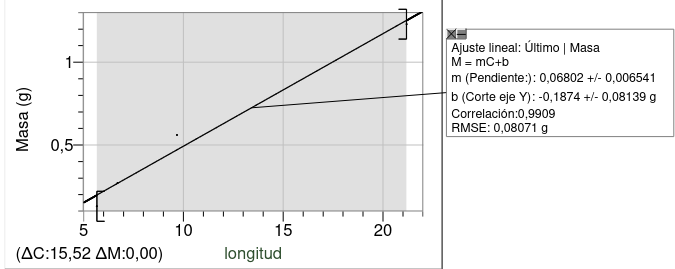
\includegraphics[width=0.9\textwidth]{Img/Figura2_Lab12.png}
    \captionof{figure}{Grafica de Masa Vs Longitud}
    \label{fig}
\end{Figura}
\begin{Figura}
    \centering
    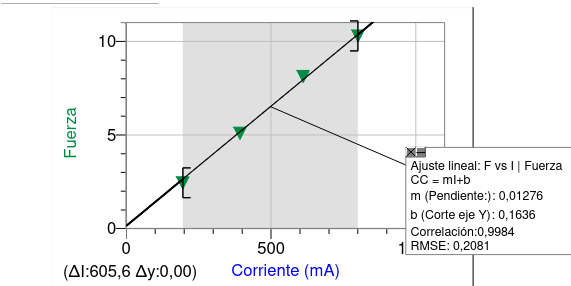
\includegraphics[width=0.9\textwidth]{Img/Figura3_Lab12.png}
    \captionof{figure}{Grafica de Corriente vs Masa}
    \label{fig}
\end{Figura}
\begin{Figura}
    \centering
    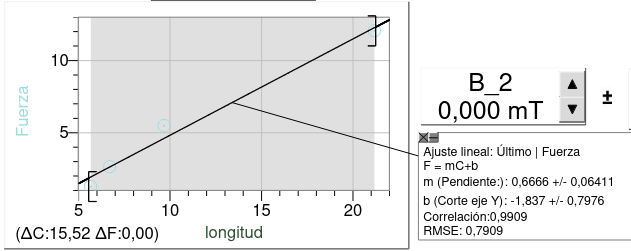
\includegraphics[width=0.9\textwidth]{Img/Figura4_Lab12.png}
    \captionof{figure}{Grafica de Corriente vs Masa}
    \label{fig}
\end{Figura}
\section{Conclusión}
En este laboratorio se quiso estudiar el efecto de un campo magnético sobre un conductor por el cual circula una corriente eléctrica. Además de determinar la relación entre la fuerza que experimenta un conductor debido a un campo magnético en función de la corriente que circula por él. En el primero de los objetivos mencionados, se vio que el efecto es el de una fuerza. Esta última se logró medir mediante la interacción del imán con el conductor. Ya que conociendo como la fuerza afectaba a una, por tercera ley de Newton, si el imán genera una fuerza sobre el conductor, el conductor genera una fuerza de igual magnitud y dirección opuesta sobre el imam. Conociendo la fuerza, pudimos junto con las 4 corrientes que calculamos, hacer una regresión lineal que nos dio la pendiente m = (0,01276 N/mA) al hacer una gráfica de F vs I (corriente). Sumado a nuestro conocimiento teórico de que la pendiente de una gráfica F vs I es m=BL(longitud) y que L = (21.18 mm), tenemos que B = m/L, 	que nos dio (0.0006G).
En un ejercicio similar, calculamos una gráfica de F vs L donde L es la longitud del conductor. Al disponer de 4 baquelas distintas hicimos una regresión sobre ellas. Pese a que no pudimos obtener datos de la baquela más pequeña en términos de fuerza. Debido a que el instrumentó de medida no tenía la suficiente precisión. De la gráfica obtenida se halló un valor de la pendiente de (0,6666 +/- 0,06411). Que junto con el hecho teórico de que B = m/I y de que se usó una corriente de 818 +/- 0.01 mA. Dio lo último un valor de campo magnético de (0.000814 G). Que es mayor al valor anteriormente obtenido.
Vale indicar, que la guía insinúa que mediríamos el campo magnético con un sensor de campo magnético. Y con el valor obtenido analizaríamos la posible discrepancia con nuestros datos hallados. Pero a nuestro grupo no se nos brindó ese sensor, he ahí que no podemos brindar errores relativos porcentuales al no tener valores ideales.
Como apéndice, decir que se trabajó con datos suministrados por compañeros. Esto último debido a que los nuestros eran inconsistentes por el motivo de una balanza mal calibrada por defecto.  
\end{multicols}
\end{document}
